%%%%%%%%%%%%%%%%%%%%%%%%%%%%%%%%%%%%%%%%%
% Simple Sectioned Essay Template
% LaTeX Template
%
% This template has been downloaded from:
% http://www.latextemplates.com
%
% Note:
% The \lipsum[#] commands throughout this template generate dummy text
% to fill the template out. These commands should all be removed when 
% writing essay content.
%
%%%%%%%%%%%%%%%%%%%%%%%%%%%%%%%%%%%%%%%%%

%----------------------------------------------------------------------------------------
%	PACKAGES AND OTHER DOCUMENT CONFIGURATIONS
%----------------------------------------------------------------------------------------

\documentclass[12pt]{article} % Default font size is 12pt, it can be changed here

\usepackage{geometry} % Required to change the page size to A4
\geometry{a4paper} % Set the page size to be A4 as opposed to the default US Letter

\usepackage{graphicx} % Required for including pictures

\usepackage{float} % Allows putting an [H] in \begin{figure} to specify the exact location of the figure
\usepackage{multirow}

\linespread{1.2} % Line spacing


%\setlength\parindent{0pt} % Uncomment to remove all indentation from paragraphs

\graphicspath{{Pictures/}} % Specifies the directory where pictures are stored

\begin{document}

%----------------------------------------------------------------------------------------
%	TITLE PAGE
%----------------------------------------------------------------------------------------

\begin{titlepage}

\newcommand{\HRule}{\rule{\linewidth}{0.5mm}} % Defines a new command for the horizontal lines, change thickness here


\center % Center everything on the page

\textsc{\LARGE   }\\[1.5cm] % Name of your university/college
\textsc{\Large No Other Than a Woman's Reason}\\[0.5cm] % Major heading such as course name
\textsc{\large Textual Analysis of Gender in Shakespeare and Elizabethan Drama}\\[0.5cm] % Minor heading such as course title

\HRule \\[0.4cm]
%{ \huge \bfseries Title}\\[0.4cm] % Title of your document
%\HRule \\[1.5cm]

\begin{minipage}{0.4\textwidth}
\begin{flushleft} \large
\emph{Author:}\\
Katherine \textsc{Roe} % Your name
\end{flushleft}
\end{minipage}
~
\begin{minipage}{0.4\textwidth}
\begin{flushright} \large
\emph{Supervisor:} \\
Prof. Bob \textsc{Berwick} % Supervisor's Name
\end{flushright}
\end{minipage}\\[4cm]

{\large
}\large May 2015 % Date, change the \ to a set date if you want to be precise

%\includegraphics{Logo}\\[1cm] % Include a department/university logo - this will require the graphicx package

\vfill % Fill the rest of the page with whitespace

\end{titlepage}

%----------------------------------------------------------------------------------------
%	TABLE OF CONTENTS
%----------------------------------------------------------------------------------------

\tableofcontents % Include a table of contents

\newpage % Begins the essay on a new page instead of on the same page as the table of contents 

%----------------------------------------------------------------------------------------
%	INTRODUCTION
%----------------------------------------------------------------------------------------

\section{Introduction} % Major section

	William Shakespeare, widely regarded as one of the best playwrights in any language, created hundreds of well-known and timeless characters of both genders. Although many thousands of books and papers have examined the role of gender in Shakespeare’s plays, very few if any have performed a rigorous quantitative analysis of the texts. For my 6.UAP project, I have performed such an analysis on the lines delivered by men versus the lines delivered by women to determine whether Shakespeare wrote male and female characters in a quantifiably distinct manner. I analyzed the number of unique words, types of speech, sentence length, line length, and sentiment of every line in 36 Shakespeare plays . Additionally, I performed the same analysis on plays by six of Shakespeare’s contemporaries in order to determine whether Shakespeare’s treatment of female characters was unique for his time or part of a broader cultural influence. My aim in this project was to write text analysis software that can be used to shed light on subtle aspects of gender treatment in Elizabethan theater and other literature.

%----------------------------------------------------------------------------------------
%	MAJOR SECTION 1
%----------------------------------------------------------------------------------------

\section{Methods} % Major section


%------------------------------------------------

\subsection{Text} % Sub-section

	The first challenge was to represent Shakespeare’s plays in a way that allowed for data analysis. I started with an HTML version of every play analyzed. I then wrote a script that converted each line into a python object. These objects included the line’s play, location in the play, location in the speech, act and scene, speaker, speaker gender, and text.
%------------------------------------------------

\subsection{Analysis}
Once the plays were prepared, I wrote a series of Python scripts to analyze the texts along several dimensions. These dimensions were number of words per line, speech length, and number of unique words. Additionally, I used natural language processing Python packages to analyze the parts of speech distribution, subjectivity, and polarity of each line.

\subsection{A Note on Categorization}
For the data analysis, I divided Shakespeare's  plays into comedies, histories, and tragedies as shown in Table 1.

\begin{center}
\begin{table}
\centering

\begin{tabular}{|l|l|l|}
  \hline
 \textsc{Comedies} & \textsc{Tragedies} & \textsc{Histories}\\
  \hline
  All's Well That Ends Well &  Antony and Cleopatra \hspace{8 mm} & King John \hspace{17 mm} \\
  \hline
  As You Like It & Coriolanus & Richard II\\
  \hline
  Comedy of Errors & Hamlet & Henry IV Part 1\\
  \hline
  Cymbeline & Julius Caesar & Henry V\\
  \hline
  Love's Labours Lost & King Lear & Henry VI Part 1\\
  \hline
  Measure for Measure & Macbeth & Henry VI Part 2\\
  \hline
  The Merchant of Venice & Othello & Henry VI Part 3\\
  \hline
  The Merry Wives of Windsor & Romeo and Juliet & Richard III \\
  \hline
  A Midsummer Night's Dream & Timon of Athens & Henry VIII \\
  \hline
  Much Ado About Nothing & Titus Andronicus & \\
  \hline
  Pericles &  & \\
  \hline
  The aming of the Shrew & & \\
  \hline
 The Tempest & & \\
  \hline
  Troilus and Cressida & & \\
  \hline
  Twelfth Night & & \\
  \hline
  Two Gentlemen of Verona & & \\
  \hline
  The Winter's Tale & & \\
  \hline
\end{tabular}
	\caption{Shakespeare Play Categorization}
\end{table}
\end{center}


	

%----------------------------------------------------------------------------------------
%	MAJOR SECTION X - TEMPLATE - UNCOMMENT AND FILL IN
%----------------------------------------------------------------------------------------

\section{Results}

\subsection{Words Per Line} % Sub-section
Shakespeare is well known for writing in iambic pentameter, meaning that, with very few exceptions, each line of his plays include ten syllables. Counting the average number of words per line, therefore, is a good measure for the average length of a spoken word. I postulated that female characters might have a higher number of average words per line, correlating to shorter words. Contrary to this expectation, men and women speak almost exactly the same number of words per line. In fact, in all the plays, men speak about 7.53 words per line compared to women's 7.41 (about a 1.6\% difference). Women consistently spoke fewer words per line than men in all three categories of play, although there were individual plays (such as Coriolanus) where the overall trend was reversed. The average number of words per line for men and women in the tragedies are shown in Figure 1.

\begin{figure}[H] % Example image
\center{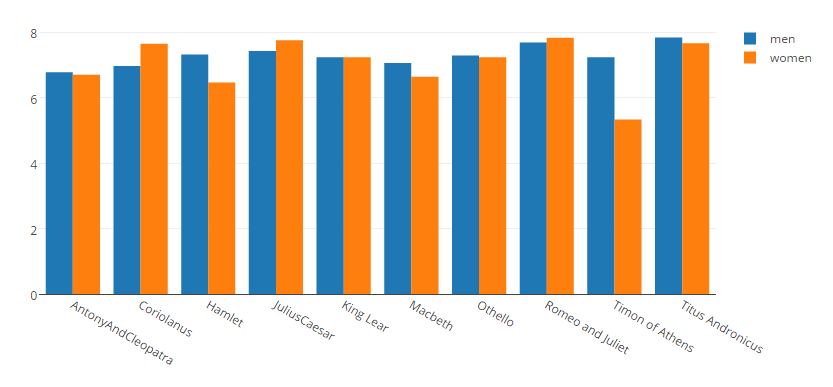
\includegraphics[width=0.8\linewidth]{wpl}}
\caption{Example image.}
\label{fig:speciation}
\end{figure}

% Content

%------------------------------------------------

%\subsection{Subsection 2} % Sub-section

% Content

%----------------------------------------------------------------------------------------
%	CONCLUSION
%----------------------------------------------------------------------------------------

\section{Conclusion} % Major section


%----------------------------------------------------------------------------------------
%	BIBLIOGRAPHY
%----------------------------------------------------------------------------------------

\begin{thebibliography}{99} % Bibliography - this is intentionally simple in this template

\bibitem[Figueredo and Wolf, 2009]{Figueredo:2009dg}
Figueredo, A.~J. and Wolf, P. S.~A. (2009).
\newblock Assortative pairing and life history strategy - a cross-cultural
  study.
\newblock {\em Human Nature}, 20:317--330.
 
\end{thebibliography}

%----------------------------------------------------------------------------------------

\end{document}